% So we make this "beamer" rather than document!

\documentclass[11pt]{beamer}
% For handout add ,handout after 11pt

\usetheme[sectionpage=none,numbering=none]{metropolis}           % Use metropolis theme
	% To do printouts, add ", handout"  after aspectratio.
\usepackage{booktabs}
\usepackage{graphicx}
\usepackage{color}

\title{Welcome to Unifying Data Science \\ \emph{(Continued)} }
\author{\small Nick Eubank}
\date{\vspace*{.3in} \date}


% This is the beginning of a real document!
\begin{document}


\begin{frame}[c]
\maketitle
\end{frame}


\begin{frame}[c]{}
    \centering 
    Part Two: Unifying Data Science
  \end{frame}
  
  \begin{frame}[c]{How did Data Science become a thing?}
  
  \begin{itemize}
      \pause \item Academic research is organized into silos:
      \pause
      \begin{itemize}
          \item Computer Science
          \item Statistics
          \item Economics
          \item Political Science
          \item Engineering
      \end{itemize}
  \end{itemize}
  \pause $\Rightarrow$ Development of new tools occurred \emph{within} each silo.
  \end{frame}
  
  
  \begin{frame}[c]{Where are we today?}
  Very little cross-pollination across silos
  \begin{itemize}
      \pause \item Lots of duplication of development.
      \pause \item Every silo has its own vocabulary.
      \pause \item Each silo has focused on the aspects most relevant to their applications. e.g.:
      \begin{itemize}
          \pause \item CS likes to classify things and make predictions, don't care how model works
          \item Social scientists like to make causal statements, don't care about predictive power
      \end{itemize}
  \end{itemize}
  \end{frame}
  
  \begin{frame}[c]{Blind Men and the Elephant}
  \pause 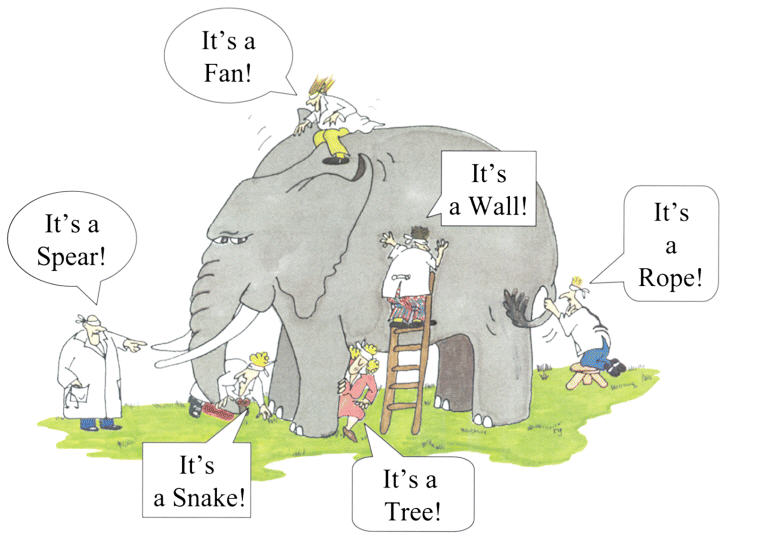
\includegraphics[width=\textwidth]{blindmenelephant.jpg}
  \pause $\Rightarrow$ This is where data science is \emph{now.}
  \end{frame}
  
  \begin{frame}[c]{What do I think Data Science should be?}
  \pause An effort to unify the development of quantitative methods \\
  \pause $\rightarrow$ Recognize the elephant
  \end{frame}
  
  \begin{frame}[c]{This Class}
  Discipline of learning how best to \alert{answer questions} using \alert{quantitative data.}
  \end{frame}
  
  \begin{frame}[c]{This Class}
  \begin{enumerate}
    \item Introduce a taxonomy of questions \\
    {\color{gray} Descriptive, causal, predictive}
    \pause \item \alert{For each class of questions}, we will discuss:
    \begin{itemize}
      \item Intrinsic challenges to answering each class of questions
      \item What tools are best suited to each type of question
    \end{itemize}
  \end{enumerate}
    \pause   By the end of the course, you should know when to reach for...
    \begin{itemize}
      \pause \item Unsupervised machine learning
      \item Supervised machine learning
      \item Range of causal inference techniques
      \item Other approaches to descriptive analysis
    \end{itemize}
  \end{frame}
  
  
  \begin{frame}[c]{This Class}
  The tool you use should be dictated by the question you seek to answer
  \end{frame}
  
  \begin{frame}[c]
    \centering
    Part Three: Your Data Science Project
  \end{frame}
  
  \begin{frame}[c]{Data Science Project}
  Over semester, you will also develop a data science project from start-to-finish
  \begin{itemize}
    \item Teams of 3-4,
    \item On topic of your own choosing.
    \item Only rule: it has to be causal.
  \end{itemize}
  \pause $\rightarrow$ Nice portfolio piece\\
  \pause $\rightarrow$ MIDS first-years: Capstone with training wheels
  \end{frame}
  
  
  \begin{frame}[c]{Data Science Project}
    Introducing in stages:
    \begin{itemize}
      \pause \item Stakeholder management 
      \pause \item Backwards Design
      \pause \item Workflow Management 
      \pause \item Presenting to Different Audiences 
      \pause \item Giving Feedback
    \end{itemize}
  \end{frame}
    
  
  \begin{frame}[c]{Who Are We?}
        I am a empirical / computational social scientist
        \begin{itemize}
            \pause \item PhD in Political Economy, Masters in Economics, BA in Economics and International Relations
        \item Research on criminal justice, policing, social networks, election administration, gerrymandering, and (in days gone by) international development. 
        \end{itemize}
        \pause (But I have a pretty strong CS background for a social scientist.)\\
      \vspace*{0.2cm}
      \pause Nathan Warren \& Becky Chen (TA) 
      \begin{itemize}
        \pause \item MIDS Second Year Students
         \item \emph{Extremely} good at this
         \pause \item Causal inference is a discipline that people spend their careers studying, so they are terrific resources, but also be aware you may hit questions they redirect to me. 
      \end{itemize}
  \end{frame}
  
  \begin{frame}[c]{Things to Know}
  \begin{itemize}
    \item Course site: \url{http://www.unifyingdatascience.org} \\
    \emph{Contents subject to change!}
    \pause \item Readings are \emph{incredibly} important. \\
    \pause \item Reading reflections for every reading. \\
    Due \textbf{Night before class.} \\
    \pause Reading quizzes are likely to be a regular feature of the class. \\
    \pause \item If you don't know git or github, you'll want to learn that early.
    \begin{itemize}
      \item Data Camp and Practical Data Science tools will be made available
      \item Workshops hosted by Library
    \end{itemize}
    \pause \item Books: 
    \begin{itemize}
      \item \emph{Mastering 'Metrics}
      \item \emph{Mostly Harmless Econometrics}
    \end{itemize}
  \end{itemize}
  \end{frame}
  
\begin{frame}
    \frametitle{If you have issues...}
    \begin{itemize}
        \pause \item With the course material,
        \pause \item With the course design,
        \pause \item With learning online,
        \pause \item With the isolation associated with COVID-life,
        \pause \item \emph{Or anything else}...
    \end{itemize}
    \pause \textbf{Talk to me!}
\end{frame}

  \begin{frame}[c]
  \centering
  Phew. That's it!   \\
  Questions?
  \end{frame}
  
\end{document}
